






%\chapter*{Part I Conclusion}{Introduction de la Partie I}
\chapter*{Conclusion de la Partie I}


% to have header for non-numbered introduction
\markboth{Conclusion}{Conclusion}


%\headercit{}{}{}


%La première conclusion marquante de cette première partie se résume parfaitement dans le meme suivant :


%{\centering
%\medskip
%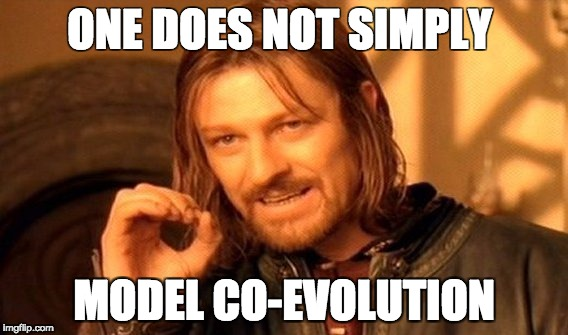
\includegraphics[width=\textwidth]{Figures/Art/onedoesnotsimply.jpg}
%\medskip
%}




\comment[JR]{here fix scales and process, and why morphogenesis and evolutive urban theory}


\begin{itemize}
	\item Retour sur la co-evol, def precise.
	\item Besoin carac empirique : annonce spatio-temp caus
	\item Inclusion dans les modeles : annonce deux streams, pourquoi.
\end{itemize}



Après cet aperçu de la littérature, incluant différents degrés de couplage entre les composantes des réseaux et territoires, nous sommes en mesure de préciser ce que nous entendrons par \emph{modéliser la co-évolution}.


Or l'interdépendance généralisée trouve vite ses limites si les motifs ne sont pas finement caractérisés. Elle permet comme prémisse épistémologique de considérer certaines ontologies et certaines démarches de modélisation, mais ne permet pas de comprendre finement la structure et les processus d'un système. Par exemple, étant donné un réseau topologique d'interaction entre entités et des motifs temporels de propagation correspondants, on peut se demander quels sont les motifs de corrélations statiques et dynamiques correspondants, s'il existe des causalités et à quelles échelles. Il existe en pratique un grand nombre de ``régimes'' de co-évolution possibles\comment[FL]{discutable}, liés à la structure du réseau écologique de la niche correspondante si on interprète celle-ci de cette façon~\cite{holland2012signals}. L'idée de diffusion hiérarchique de l'innovation dans la théorie évolutive capture par exemple qualitativement certains de ces aspects, mais la quantification des régimes correspondants et donc de la co-évolution reste une question ouverte.


L'une de nos contributions principales\comment[FL]{c'est un point important qui se trouve un peu dilue ici} est sous forme théorique en~\ref{sec:theory}. Il s'agira de clarifier cette notion et d'en donner une définition précise.


A ce stade, l'état de l'art fait ci-dessus témoigne d'une faiblesse de la littérature dans le domaine du couplage fort entre évolution des territoires et croissance des réseaux, vu la portée restreinte et la disparité des travaux revus. Les lacunes à combler sur ce point seraient donc liées à l'introduction de modèles fortement couplés dans le temps plus ou moins multi-processus et multi-échelles, pour lesquels une partie des modèles décrits ci-dessus sont précurseurs.






% why does not study mobility et suggestion preliminaire de meso-macro scales only. -> conclusion Partie I

%\bpar{}
%{
%Il faut aussi garder à l'esprit que le transport en lui-même est différent des réseaux de transport\comment[FL]{en quoi estce un argument ?}, puisqu'il correspond à l'utilisation de ceux-ci par les agents territoriaux. Dans une grande partie des approches que nous décrirons par la suite, et typiquement les approches appliquée en planification urbaine, la modélisation du transport s'axe sur des question de demande, d'offre, de congestion, c'est à dire à des échelles relatives à la mobilité, et est liée au réseau mais ne se concentre pas directement sur celui-ci\comment[FL]{ce n'est pas clair $\rightarrow$ la croissane du reseau ?, l'usage du reseau ? la croissance de l'usage du reseau ?} comme notre positionnement propose\comment[AB]{$\simeq$}.
%}


